\section{Learning MPIs}\label{sec:learning-mpis} 

Some of the major challenges in high-quality novel view synthesis include synthesizing pixels occluded in one or more of the provided views, disentangling and localizing ambiguous pixels at/near the boundaries of foreground and background objects, localizing pixels at transparent, translucent, reflective, or texture-less surfaces, etc. Moreover, whereas interpolating novel views at desired viewpoints lying amidst given views is easier to achieve than extrapolating significantly beyond the baselines (distances between camera centers) of input viewpoints, these challenges can emerge in either case. So far, it has been found that learning view synthesis is the way to go for tackling them all in one shot.

Before the Machine Learning (ML) boom in Computer Vision (CV) circles in 2012, convolutional filters had to be handcrafted and dexterously layered one atop the other before input views could be subjected to them and various types of features could be extracted in the process of rendering novel views. All the aforementioned view synthesis challenges had to be manually targeted by way of devising various combinations of these filters. This meant a high proportion of artifacts induced in novel views could be left unresolved. Since the time that the efficacy of CNNs in CV was proven by Krizhevsky, Sutskever, and Hinton~\cite{krizhevsky_imagenet_2012} in 2012, to the delight of the CV community, the need to handcraft filters was obviated by ML models that learned to design all required convolutional filters on their own in their various hidden layers. These self-taught filters are defined by the weights and biases in each hidden layer neuron. The weights and biases constantly improve during training and the convolutional filters defined by them are specific to the datasets they are trained on, with some degree of generalizability to other datasets. If trained well under effective hyperparamter tuning, learned filters can evolve to surpass manual filters in redressing occlusion, transparency, reflection, and other image synthesis problems.

View synthesis lends itself to being a semi-well-posed to well-posed learning problem where two or more images of a scene can be shot and an ML model can be exposed to one of more of these images while being expected to predict one or more of the remaining views that have been withheld from it. The quantitative difference between the corresponding predicted and withheld (as ground truth) views will then be the loss that the ML training seeks to minimize. Since end-to-end view synthesis without an intermediate representation is still largely unrealized, the popular way to synthesize novel views is to learn an intermediate representation of the scene common to the input views and use this intermediate representation to render novel views. The MPI intermediate representation has proven to be one the most effective representations for this purpose with implications as significant as real-time high-quality view synthesis.

\subsection{Seminal Work}\label{subsec:seminal-work}

The roots of the MPI representation may be traced back to seminal papers such as 1996's Collins~\cite{collins_space-sweep_1996}, 1998's Shade et al.~\cite{shade_layered_1998}, and 1999's Szeliski and Golland~\cite{szeliski_stereo_1999}. Collins perfected the concept of Plane Sweep Volumes (PSVs), Shade et al. introduced layered depth images, and Szeliski and Golland introduced the actual MPI representation itself. These groundbreaking techniques have also been compared in Scharstein and Szeliski~\cite{scharstein_taxonomy_2002}. 

\begin{figure}[!h]
    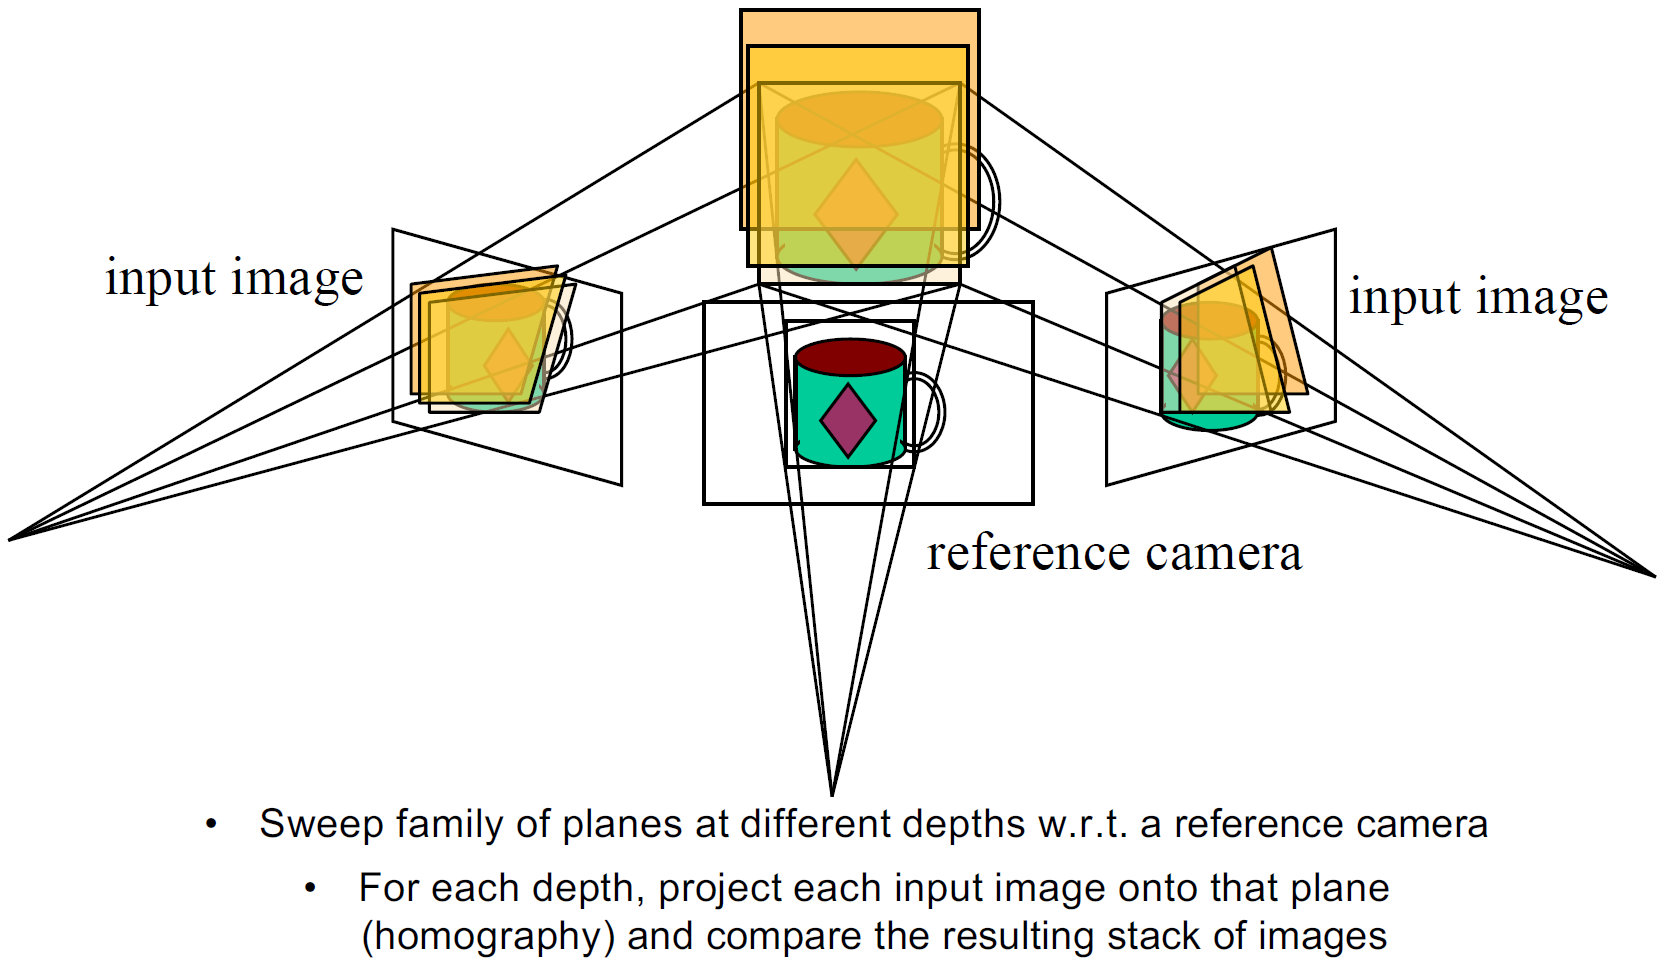
\includegraphics[width=1\columnwidth]{figures/plane-sweep-volume.png}
    \caption{Plane Sweep Volume Representation~\cite{svetlana_2019}}
    \label{fig:plane-sweep-volume}
\end{figure}

Collins~\cite{collins_space-sweep_1996} applied the PSV representation to the problem of reconstructing the 3D scene from multiple views while simultaneously performing feature matching across all views sharing common features. Feature matching is the process of matching corresponding ``features of interest" characterized by their repeatability across multiple views of the same world scene. Examples include keypoints, corners, edges, objects, etc. Matched views can be rectified and used for triangulating depth, etc., as mentioned in section~\ref{sec:motivation}. In the author's implementation, instead of going for a resource-intensive 3D representation that would require splitting the entire 3D scene space into voxels and reprojecting\footnote{projecting to a target plane by unapplying and applying the homographies needed to project to the source and target planes, respectively, while accounting for surface normals, plane offsets, camera rotations and translations, etc., as described in subsection~\ref{subsec:base-papers}} all feature points from all views in such manner that the reprojected light rays passed through this uniformly partitioned space, he sampled the 3D scene space at various 2D planes along the depth ($z$) axis as if capturing just one 2D plane sweeping though it at various instants in time. He partitioned the sweeping plane into cells and allowed each reprojected light ray to vote for a group of cells that fell within a certain radius of the point of intersection of the light ray with the plane. This accounts for the fact that rays from corresponding feature points across all views may not converge most of the time due to projection errors. He then chose the z-coordinate of the sampled plane containing the cell with the maximum votes for a feature point to be the z-coordinate of the feature point in the world scene. The $x$ and $y$ world coordinates would be defined by the victor cell. The winning cell would also determine the 2D feature point correspondences simultaneously just by virtue of the converging rays being retraced to their respective originating views. PSVs, in their various reimplemented forms, have almost become synonymous of layered volumetric representations these days (Figure~\ref{fig:plane-sweep-volume}).

Shade et al.'s~\cite{shade_layered_1998} Layered Depth Image (LDI) scene representation is similar to MPI scene representation in that both MPI and LDI consist of a series of fronto-parallel planes facing a chosen reference viewpoint and placed at varying depths from it. These planes contain the RGB information of the original pixels of the scene's image(s), ssegregated according to depth. MPI differs from LDI in that it has alpha masking effects at each layer, as it is generated with alpha transparency maps for each layer. Also, MPI has fixed depths for each layer as opposed to the variable layer depths of LDI. But in both cases, by virtue of layering, users are able to experience a simulation of what happens when they move their heads while looking at a scene in the world --- they are able to look around foreground objects that occlude background ones. 

Szeliski and Golland~\cite{szeliski_stereo_1999} first introduced the MPI representation for purposes of stereo matching with simultaneous RGBA estimation at each matched pixel. Stereo matching, otherwise called disparity mapping, uses feature matching techniques like SIFT\footnote{Scale-Invariant Feature Transform~\cite{lowe_distinctive_2004}} in pixel-and-sub-pixel-wise disparity estimation for 3D scene reconstruction from rectified stereo images. The authors' framework was the first to extract high-accuracy depth, color, and transparency maps for several images at a time, operating even at sub-pixel levels. They were able to enforce sub-pixel accuracy and perform effective matte separation of foreground and background elements despite the usual 3D vision challenges such as occlusions, etc., because they came as close to modern ML reimplementations as possible. They implemented various loss functions such as a pixel-wise weighted photometric L1 norm between the input and reprojected images, a per-pixel smoothness constraint on the RGBA values allowed in the reprojected images, etc. They then performed an iterative refinement of the estimated RGBA values with the help of a gradient descent algorithm designed to optimize a combination of all these losses, but sans the explosive power of neural networks.

\subsection{Influential Work}\label{subsec:influential-work}

Flynn et al.~\cite{deep_stereo_2016} is the first to apply CNNs in an end-to-end manner to novel view synthesis from diverse collections of indoor and outdoor imagery in the wild provided camera parameters\footnote{camera intrinscics such as focal length and principal point and camera extrinsics/pose such as position and orientation} are available for each image. Their paper describes why it would be unwise to expect any CNN to synthesize novel views without being provided with the pose of each given view as well --- the network would have to learn epipolar geometry itself! Epipolar geometry --- the geometry of binocular and multi-view stereo vision --- gives us the epipolar constraint $x'^T F x = 0$ between all corresponding points $x$ and $x'$ in a stereo pair. Here, $F$ is called the fundamental matrix and is derived from the intrinsic and extrinsic parameters of the stereo cameras involved. To circumvent such an indeterminate and expensive pixel-to-pixel training scenario, the authors had PSVs (Figure~\ref{fig:plane-sweep-volume}) come to the rescue. They supplied all input views required to synthesize a novel view as separate PSVs to their network. Each input plane sweep would contain all pixels of the respective input view reprojected onto a chosen number of planes at chosen depths in the usual ``stack of acetates" manner with the panes all having their viewpoints match with the novel view's. The planes that each RGB pixel is reprojected onto will also determine the availability of the pixel (as alpha values ranging from 0 to 1) to the surrounding voxels of the PSV. The plane sweep of each input view has the pose information of the view implicitly encoded in it by virtue of its construction. Moreover, the planes sweeps of all input views of the same scene trivially enforce the epipolar constraint as matching pixels across all these inputs may be located in the same depth-wise column of each plane sweep. Each of these depth-wise columns may then be computed upon by the network independently of other columns in producing the corresponding novel pixel.

They train the error function

The authors' method currently requires reprojecting each input image to a set of depth planes; the authors currently use 96 depth planes, which limits the resolution of the output images that the authors can produce. Increasing the resolution would require a larger number of depth planes, which would mean that the network takes longer to train, uses more RAM and takes longer to run. This is a drawback shared with other volumetric stereo methods; the method requires reprojected images per rendered frame, rather than just once when creating the scene. The authors plan to explore pre-computing parts of the network and warping to new views before running the final layers

The traiing error function is the one that is constanly being learnt by the network

Both Flynn et al. and Kalantari et al. are unable to train with entire images at a time, instead they extract patches of training images and
Moreover It was also the first to create a common scene representation  
for the rest real time rendering is a challenge

 The authors seek a scene representation that can be predicted once given a pair of input views and then reused to predict a large number of output views, in contrast to past work that required prediction of each output view independently.

What also comes close to the MPI representation is the layered repesentaion of Pennar and Zang but then again in all these methods they predict one rep for one targer view tp be renderd 

Some more MPI-related papers released between Zhou et al and Tucjer and carsloi n are 
They are a great reading which explore different directions that you might find interesting, finetning it single-view MPIs 
(Pushing the Boundaries, DeepView, Local Lightfield Fusion)  but none of them are tackling the single-view approach so you won't need to understand them in detail.


\subsection{Base Papers}\label{subsec:base-papers}

Zhou et al.~\cite{zhou2018stereo} was the first to implement view extrapolation to significantly larger baselines (up to 8x input baselines) than prior work. They use a stereo pair of images to learn an MPI prediction network in the following manner:

\begin{itemize}
    \item The camera parameters $c_1\ =\ (p_1,\ k_1)$ and $c_1\ =\ (p_2,\ k_2)$ of the stereo pair, $(I_1,\ I_2)$, are also needed for the prediction process, along with the target image $I_t$ and its parameters $c_t$. Here, $p_i$ and $k_i$ are the camera extrinsics and intrinsics of the respective images.
    \item The viewpoint of one image of the stereo pair, $I_1$, is used as the reference viewpoint for the MPI to be predicted at. Hence, $p_1$ would be an identity matrix.
    \item The goal is to learn a network that generates an MPI representation with inputs $(I_1,\ I_2,\ c_1,\ c_2)$ such that when the MPI is rendered at viewpoint $c_t$, it would produce the target image $I_t$. 
    \item As demonstrated by Flynn et al.~\cite{deep_stereo_2016}, an effective way to encode pose information for training is via a PSV. Hence, the input to their customized encoder-decoder type network includes a PSV version of $I_2$ $(\hat{I_2})$ with the planes reprojected into the final MPI's viewpoint, $c_1$, and with the entire plane sweep concatenated with the regular version of $I_1$. The depth planes of $\hat{I_2}$ are also chosen to coincide with the ones of the output MPI.
\end{itemize}

\begin{figure}[!h]
    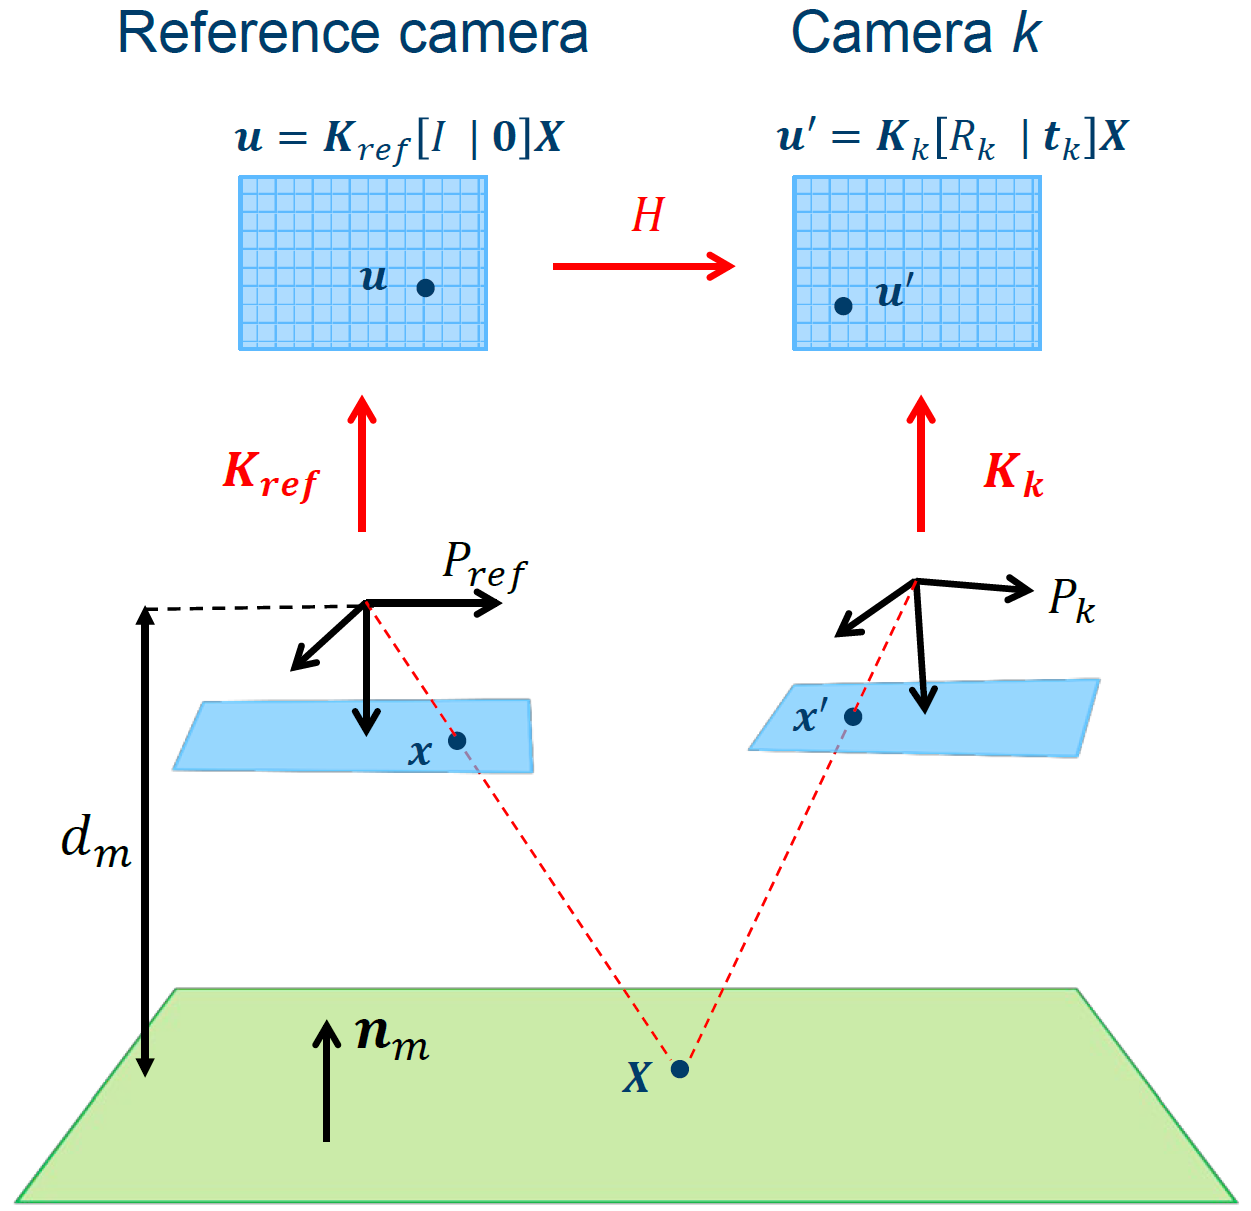
\includegraphics[width=0.75\columnwidth]{figures/standard-inverse-homography.png}
    \caption{Standard Inverse Homography or Reprojection~\cite{brann_forelesninger_2016}}
    \label{fig:standard-inverse-homography}
    {\small Here, the 3D point $\mathbf{X}$ on the MPI plane in the world is the \textit{homogeneous} version (determined up to scale) of its projection $\mathbf{x}$ on the reference camera's image plane in camera coordinates, i.e., with the camera's image plane centered at the camera center, $P_{ref}$. More precisely, $\mathbf{X} = [X,Y,d_m]^T \sim \tilde{\mathbf{x}} = [X/d_m,Y/d_m,1]$. This is because all MPI world planes are fronto-parallel to the reference camera and their equations can be given by $\mathbf{n_m \cdot \tilde{x}} + a = 0$, where $\mathbf{n_m} = [0,0,1]$ is the plane normal and $a = -d_m$ is the plane offset from $P_{ref}$. The projection $\mathbf{u}$ on the reference camera's image plane in regular image coordinates is attained by applying reference camera intrinsics $\mathbf{K_{ref}}$ to $\mathbf{x}$. Since the MPI is not necessarily fronto-parallel to the target camera $P_k$, $\tilde{\mathbf{x'}}$ need not be $[X/d_m,Y/d_m,1]$ even though $\mathbf{X} \sim \tilde{\mathbf{x'}}$ as well. $\mathbf{u'}$ and $\mathbf{K_k}$ similarly belong to the target camera, as does target camera pose $[R_k|\mathbf{t_k}]$. The world plane \textit{induces} the homography $H = \mathbf{K_k} (R_k - \mathbf{t_k} \mathbf{n_m}^T / a) \mathbf{K_{ref}}^{-1}$ between the image planes of $P_{ref}$ and $P_k$, so we can go from $\mathbf{u}$ to $\mathbf{u'}$. To go from $\mathbf{u'}$ back to $\mathbf{u}$, we'd use $H^{-1}$~\cite{zikuicai_derivation_2019}.}  
\end{figure}

The 3D structure of the scene depicted by $I_1$ and $I_2$ is automatically learnt by the network by merely being able to compare $I_1$ with each of the reprojected images of $I_2$ in the input stack $(\hat{I_2^1},\ \hat{I_2^2},\ \ldots,\ \hat{I_2^D},\  I_1)$, where $D$, again, refers to the total number of MPI depth planes (Section~\ref{sec:motivation}). In order to reduce resource consumption due to network over-parameterization, the network's initial outputs do not consist of separate RGBA maps for each MPI layer but rather just a ``background" image intended to capture pixels occluded in $I_1$ and a set of color blending weight maps and alpha maps for each MPI layer. The actual RGB values in each layer, $C_d$, are then easily computed by taking the per-pixel weighted average of $I_1$ and the predicted background image $\hat{I_b}$:

\[ C_d = w_d \odot I_1 + (1 - w_d) \odot \hat{I_b} \]

Here, $\odot$ refers to the Hadamard product and $w_d$ refers to the RGB blending weights from the initial network output, specific to MPI layer $d$. The rest of the training pipeline consists of the rendering of the MPI at the target viewpoint, $c_t$, and the gradient descent algorithm involving a VGG perceptual (similar to LPIPS~\cite{zhang_unreasonable_2018}) loss function between the rendered view and ground-truth target view. Rendering an MPI first involves warping each RGBA MPI layer onto the target camera's image plane using the standard inverse homography or reprojection operation~\cite{hartley_multiple_2004}, as illustrated in figure~\ref{fig:standard-inverse-homography}. But, anticipating usual reprojection errors, they resample each pixel to be warped by bilinear interpolation with respective four-grid neighbors. These rerendered MPI layers are then alpha-composited in back-to-front order to get the final predicted target view. All in all, the authors' implementation was ingenious in a number of ways from training to predict novel views at varying distances from input views so as not to overfit to predicting only up to a limited number of baselines, to their use of assorted but apt convolutional layers like dilated convolutions and fractianllly-strided convlutions ansd covolutions witjh skk pconnectoisn, and to econstruct object stucture and texture details better in synthesized view swith by using VGG perceptioual lsoss. and to not depend on just struture fromm motion pipelines but as well as using ORB slam 2 to estimate the inital views. Moreover, they were meticulous in their dataset creaton process when they created the RdealEstate10K dataset use of ORB slam 2 before strucrture from motion pipelins like COLMAP  

Depth maps are derived from the predicted MPIs and not predicted in parallel with the MPIs

 \subsection{The 2020 paper}\label{subsec2:2020}

Taking a photograph and being able to move the camera around is an enticing way to bring a scene to life. It requires an understanding of the scene's three-dimensional structure, reasoning about occlusions and what might be behind them, and rendering high-quality, spatially consistent new views in real time. The authors use the multiplane image (MPI) representation, which is capable of modeling disocclusions and non-Lambertian effects, generates spatially consistent views, is well-suited for creation via convolutional networks, and can be rendered efficiently in real time [37]. A special issue occurs when overseeing such a system via view synthesis, due to the uncertainty in the input data's global scale. The authors address this issue with a method of scale invariant view synthesis that makes use of sparse point sets generated during the training data generation process. The authors present an edge-aware smoothness loss that prevents depth maps created from predicted MPIs from becoming excessively fuzzy, even in the absence of depth supervision.

While the authors' purpose is view synthesis rather than depth prediction, they can easily generate disparity maps from the MPIs and use these to assess depth performance. The authors conduct quantitative and qualitative evaluations of the approach using the RealEstate10K dataset, as well as in-depth evaluations using the iBims-1 benchmark and comparisons to earlier view synthesis methods using the Flowers and KITTI datasets. The authors demonstrate the ability to predict MPIs for view synthesis from single image inputs without the need for ground truth 3D or depth information, and they introduce a scale-invariant approach to view synthesis that enables them to train on data with scale ambiguity, such as that derived from online video. A possible next path would be to combine MPI prediction with adversarial losses to determine whether it is possible to produce better, and more realistic, inpainting.


In the abstract they say they use scale-invariant view synthesis as supervision by which they mean they use additional views of the scene  as supervision (possibly unscaled?)


Single-view view synthesis only during inference. During training 2020 model learns to predict an MPI in one stage without requiring any post-processing steps but nevertheless requires multiple images of the same scene as supervision in the one-stage training pipeline.

Single view view synthesis is an diffenert fromo the data collection aspedct of the 2018 paper becasue they retain the sparse point clouds and a record of whicvh points were tracked in each frame (refereed to as vidsible points)


how do they even come up with depth pixels for both LDI/MPI? do they already know depth from ground truth ????
and how do they calculate depth ???

we can give the number of layers to the network - does it make a difference? 
when you have more layers you get more depth info - more clarity in the rendered image -


somehow quantizing the depths 
tyhe 3d objecxt wiil fall in different plab=nes

why did they include colmap point could vs 


\begin{figure}[!h]
    \includegraphics[width=1\columnwidth]{figures/}
    \caption{Fronto-parallel planes in MPI layered representation}
    \label{fig:mpi-layered-representation}
\end{figure}
Fig 3. Example of fronto-parallel planes

However, in fact, the coordinates of picture dots cannot be determined with arbitrarily high precision. Rather than that, other sources of noise, such as geometric noise caused by lens distortion or interest point recognition mistake, cause inconsistencies in the picture coordinates that are measured. As a result, the lines created by the associated picture points do not always meet in three-dimensional space. The objective is then to identify a three-dimensional point that fits the observed picture points optimally. Numerous approaches exist in the literature for how to define optimality and how to determine the optimal 3D location. Due to the fact that the various approaches are based on distinct optimality criteria, they generate significantly varied estimations of the 3D point x when noise is present.